%%%%%%%%%%%%%%%%%%%%%%%%%%%%%%%%%%%%%%%%%
% Beamer Presentation
% LaTeX Template
% Version 1.0 (10/11/12)
%
% This template has been downloaded from:
% http://www.LaTeXTemplates.com
%
% License:
% CC BY-NC-SA 3.0 (http://creativecommons.org/licenses/by-nc-sa/3.0/)
%
%%%%%%%%%%%%%%%%%%%%%%%%%%%%%%%%%%%%%%%%%

%----------------------------------------------------------------------------------------
%	PACKAGES AND THEMES
%----------------------------------------------------------------------------------------

\documentclass{beamer}

\mode<presentation> {

% The Beamer class comes with a number of default slide themes
% which change the colors and layouts of slides. Below this is a list
% of all the themes, uncomment each in turn to see what they look like.

%\usetheme{default}
%\usetheme{AnnArbor}
%\usetheme{Antibes}
%\usetheme{Bergen}
%\usetheme{Berkeley}
%\usetheme{Berlin}
%\usetheme{Boadilla}
%\usetheme{CambridgeUS}
%\usetheme{Copenhagen}
%\usetheme{Darmstadt}
%\usetheme{Dresden}
%\usetheme{Frankfurt}
%\usetheme{Goettingen}
%\usetheme{Hannover}
%\usetheme{Ilmenau}
%\usetheme{JuanLesPins}
%\usetheme{Luebeck}
\usetheme{Madrid}
%\usetheme{Malmoe}
%\usetheme{Marburg}
%\usetheme{Montpellier}
%\usetheme{PaloAlto}
%\usetheme{Pittsburgh}
%\usetheme{Rochester}
%\usetheme{Singapore}
%\usetheme{Szeged}
%\usetheme{Warsaw}

% As well as themes, the Beamer class has a number of color themes
% for any slide theme. Uncomment each of these in turn to see how it
% changes the colors of your current slide theme.

%\usecolortheme{albatross}
%\usecolortheme{beaver}
%\usecolortheme{beetle}
%\usecolortheme{crane}
%\usecolortheme{dolphin}
%\usecolortheme{dove}
%\usecolortheme{fly}
%\usecolortheme{lily}
%\usecolortheme{orchid}
%\usecolortheme{rose}
%\usecolortheme{seagull}
%\usecolortheme{seahorse}
%\usecolortheme{whale}
%\usecolortheme{wolverine}

%\setbeamertemplate{footline} % To remove the footer line in all slides uncomment this line
%\setbeamertemplate{footline}[page number] % To replace the footer line in all slides with a simple slide count uncomment this line

%\setbeamertemplate{navigation symbols}{} % To remove the navigation symbols from the bottom of all slides uncomment this line
}

\usepackage{graphicx,caption} % Allows including images
\usepackage{booktabs} % Allows the use of \toprule, \midrule and \bottomrule in tables
\usepackage[utf8]{inputenc} %für ß
\usepackage{subfigure}
\usepackage{amsmath} 
\usepackage[ngerman,english]{babel}

%----------------------------------------------------------------------------------------
%	TITLE PAGE
%----------------------------------------------------------------------------------------

\title[Convolutional Neural Networks]{Bilderkennung mit Convolutional Neural Networks} % The short title appears at the bottom of every slide, the full title is only on the title page

\author{Ivo Tremel und Lennard Nöhren} % Your name
\institute[CHI] % Your institution as it will appear on the bottom of every slide, may be shorthand to save space
{
Leibniz Universität Hannover \\ % Your institution for the title page
\medskip
%\textit{john@smith.com} % Your email address
}
\date{18. Januar 2018} % Date, can be changed to a custom date

\begin{document}

\begin{frame}
\titlepage % Print the title page as the first slide
\end{frame}

\begin{frame}
\frametitle{Overview} % Table of contents slide, comment this block out to remove it
\tableofcontents % Throughout your presentation, if you choose to use \section{} and \subsection{} commands, these will automatically be printed on this slide as an overview of your presentation
\end{frame}

%----------------------------------------------------------------------------------------
%	PRESENTATION SLIDES
%----------------------------------------------------------------------------------------

%------------------------------------------------
\section{Convolutional Neural Network} % Sections can be created in order to organize your presentation into discrete blocks, all sections and subsections are automatically printed in the table of contents as an overview of the talk
%------------------------------------------------

\subsection{Convolutional Layer} % A subsection can be created just before a set of slides with a common theme to further break down your presentation into chunks

\begin{frame}
	\frametitle{Covolutional Layer}
	 \begin{itemize}
		\item Diskrete Faltung auf dem Eingabebild
		\item 5x5 Matrix läuft über das Bild und filtert die Werte
		\item Matrix heißt Filterkernel
		\item Betrachtung der lokalen Umgebung
		\item Features können aus mehreren Punkten bestehen
	\end{itemize}
	
\end{frame}

%------------------------------------------------

\subsection{Pooling Layer}

\begin{frame}
	\frametitle{Pooling Layer}
	\begin{itemize}
		\item Fassen den Output von vorhergehenden Neuronen zusammen
		\item Bei MaxPooling wird der größte Wert durchgeschaltet
		\item Andere Werte werden verworfen
		\item Reduktion der Datenmenge ermöglicht schnellere Berechnung
	\end{itemize}
\end{frame}

\begin{frame}
	\frametitle{Aufbau}
	\begin{figure}
		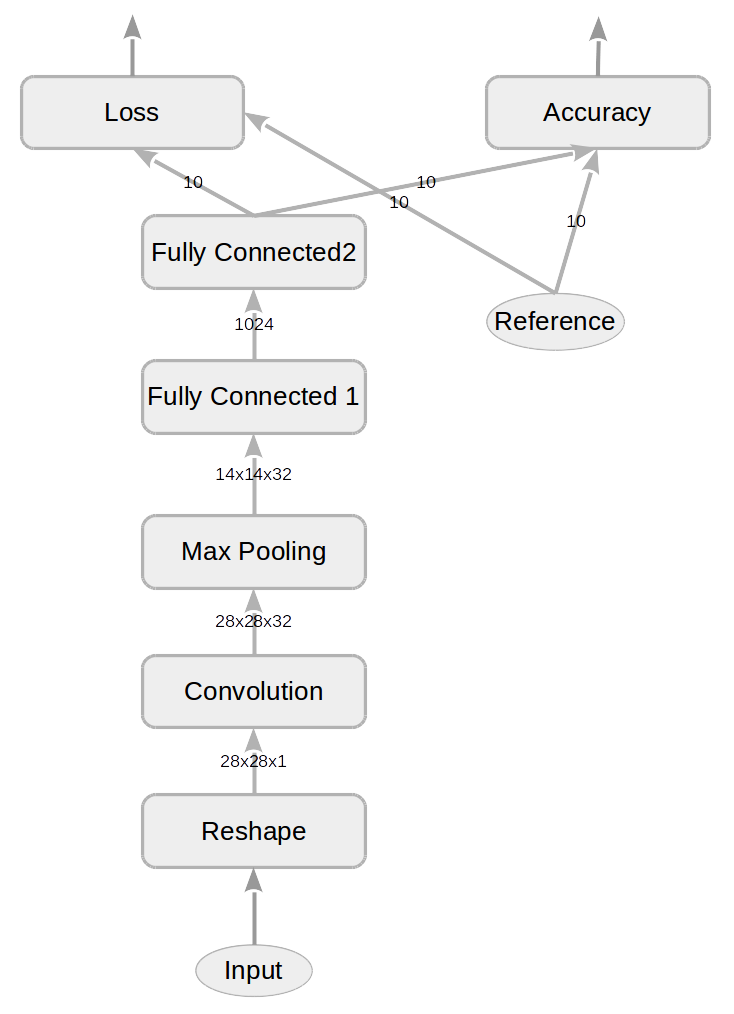
\includegraphics[width=0.4\linewidth]{images/main_graph_conv_reduced.png}
		\caption{Aufbau klassisches CNN}
		\label{fig:main_graph_conv}
	\end{figure}
\end{frame}

%------------------------------------------------
\section{Inception Module}
%------------------------------------------------

\begin{frame}
	\frametitle{Inception Module}
	\begin{figure}
		
\includegraphics[width=0.8\linewidth]{images/inception_meme.jpg}\\
		\hspace*{0pt}\hbox{\scriptsize Quelle:\thinspace{\small\itshape http://knowyourmeme.com/memes/we-need-to-go-deeper}}
		\label{fig:inception_meme}
	\end{figure}
	
\end{frame}

\begin{frame}
	\frametitle{Inception Module}
	\begin{columns}[c]
		\column{0.5\textwidth}
		\begin{itemize}
			\item Analyse des Inputs in verschiedenen Skalierungen
			\item Für niedrige Level 1x1 Convolution für kleine Features
			\item 3x3 und 5x5 Convolution für größere Features
			\item Max Pooling sehr effektiv in CNN's \\ 
			$\rightarrow$ Als Alternativer Pfad zu Convolutions enthalten
		\end{itemize}
		
		\column{0.5\textwidth}
		\begin{figure}
			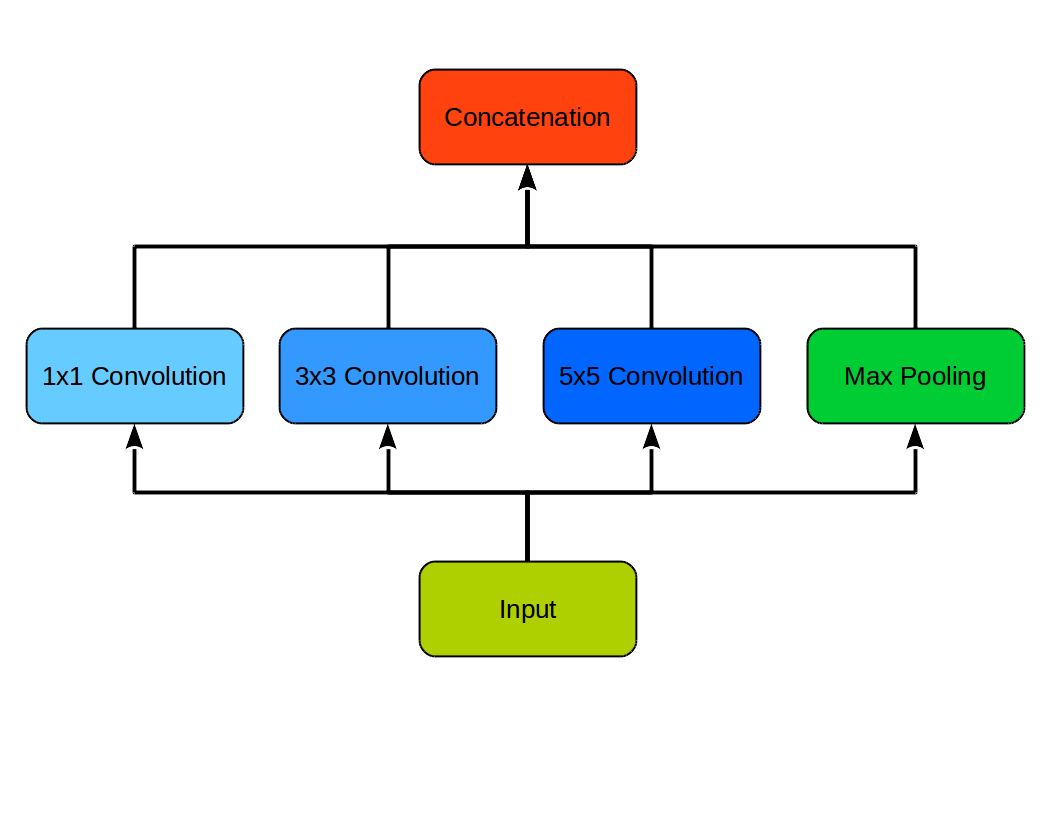
\includegraphics[width=\linewidth]{images/inception_naive_graph.png}
			\caption{Aufbau Inception Module}
			\label{fig:naive_inception}
		\end{figure}
	\end{columns}
\end{frame}

\begin{frame}
	\frametitle{Inception Module}
	\begin{columns}[c]
		\column{0.5\textwidth}
		\begin{itemize}
			\item Sehr hoher Rechenaufwand
			\item Dimension steigt stark an
			\item Deshalb: 1x1 Convolutions vor den größeren Modulen
			\item Reduziert die Dimension des Inputs
			\item Ermöglicht mehrere Inception Module in Folge 
		\end{itemize}
		
		\column{0.5\textwidth}
		\begin{figure}
			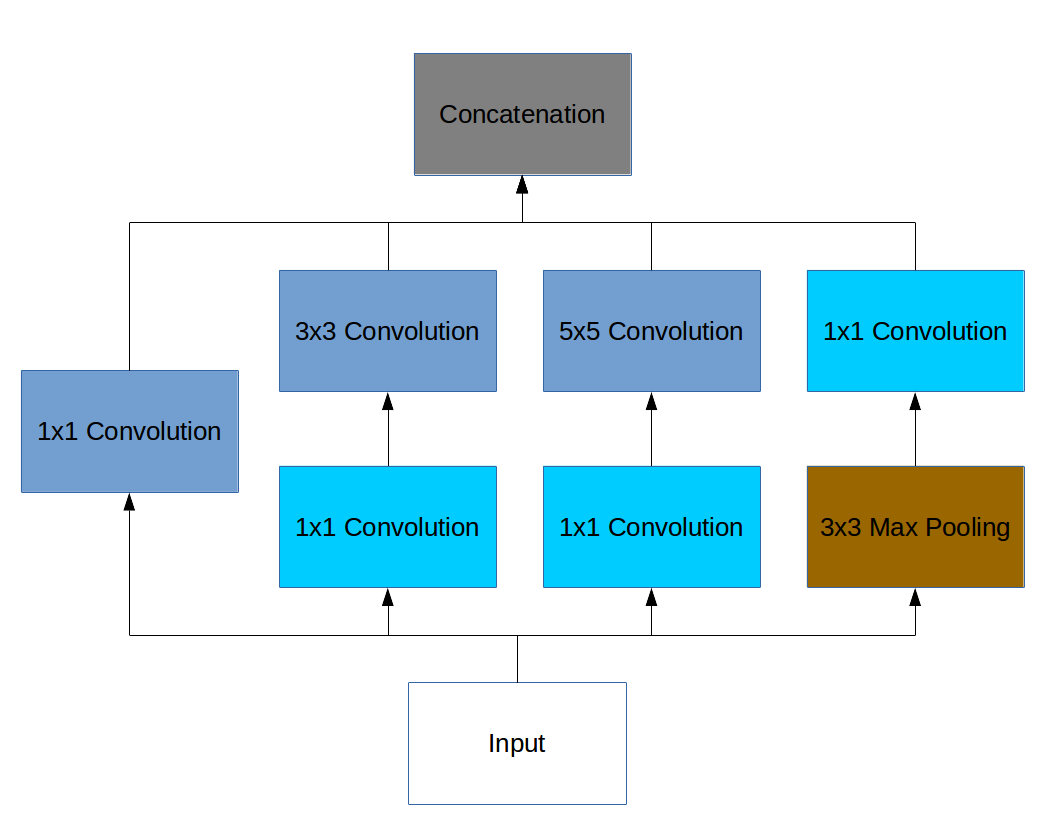
\includegraphics[width=\linewidth]{images/inception_pro_graph.png}
			\caption{Aufbau verbessertes Inception Module}
			\label{fig:pro_inception}
		\end{figure}
	\end{columns}
\end{frame}

\begin{frame}
	\frametitle{Aufbau}
	\begin{figure}
		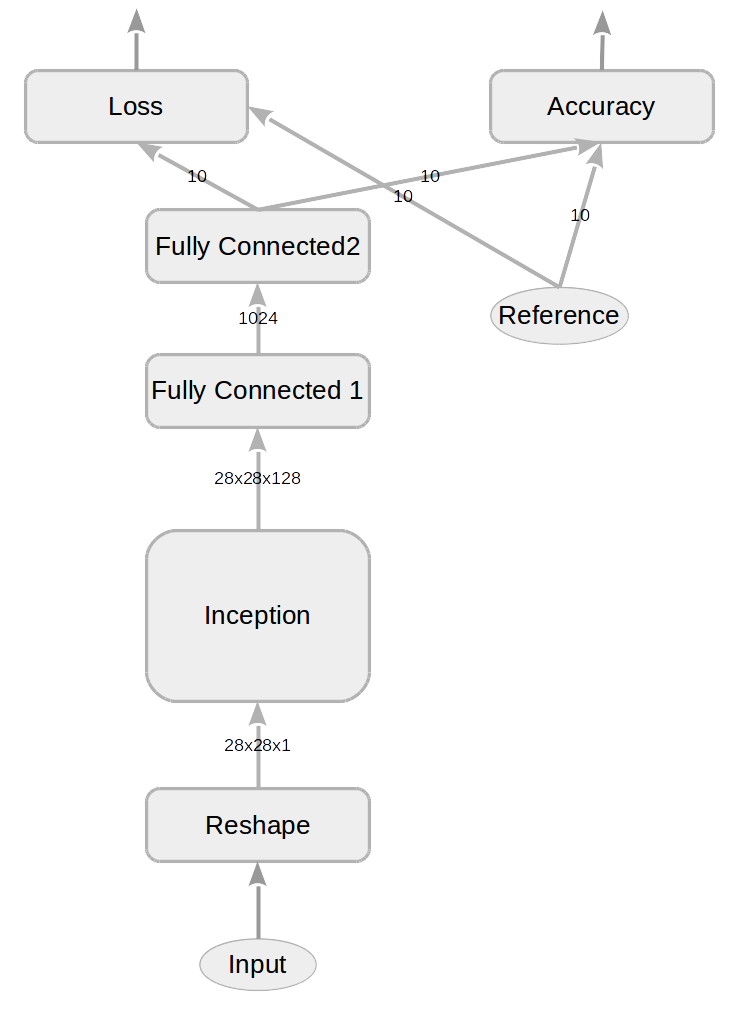
\includegraphics[width=0.4\linewidth]{images/main_graph_inception_reduced.png}
		\caption{Aufbau CNN mit Inception Layer}
		\label{fig:main_graph_inception}
	\end{figure}
\end{frame}

%------------------------------------------------
\section{Datensatz}
%------------------------------------------------

\begin{frame}
	\frametitle{Datensatz}
	\begin{itemize}
		\item 1000 Handschriftliche Buchstaben aus 10 Klassen
		\item Buchstaben A M O T U Y V und Umlaute Ä Ö Ü
		\item Einige falsche gelabelte Bilder
	\end{itemize}
	\begin{figure}
		%
\includegraphics[width=0.2\textwidth]{hand_images/image_Ae_up_106_point_24.png}
		\subfigure{
\includegraphics[width=0.15\textwidth]{hand_images/image_Ae_up_106_point_24.png}}
		\subfigure{
\includegraphics[width=0.15\textwidth]{hand_images/image_M_up_9_point_94.png}}
		\subfigure{
\includegraphics[width=0.15\textwidth]{hand_images/image_O_up_5_point_14.png}}
		\subfigure{
\includegraphics[width=0.15\textwidth]{hand_images/image_T_up_29_point_14.png}}
		\subfigure{
\includegraphics[width=0.15\textwidth]{hand_images/image_U_up_31_point_328.png}}
		\subfigure{
\includegraphics[width=0.15\textwidth]{hand_images/image_Ae_up_142_point_31.png}}
		\subfigure{
\includegraphics[width=0.15\textwidth]{hand_images/image_Oe_up_157_point_17.png}}
		\subfigure{
\includegraphics[width=0.15\textwidth]{hand_images/image_Ue_up_132_point_13.png}}
		\subfigure{
\includegraphics[width=0.15\textwidth]{hand_images/image_Y_up_46_point_8.png}}
		\subfigure{
\includegraphics[width=0.15\textwidth]{hand_images/image_V_up_46_point_314.png}}	
		\caption{Beispiele für Buchstaben aus dem Datensatz}
		\label{fig:charexample}
	\end{figure}
\end{frame}

\begin{frame}
	\frametitle{Falsch gelabelter Buchstabe}
	\begin{itemize}
		\item \glqq image\_Ä\_up\_106\_point\_24.png\grqq
	\end{itemize}
	\begin{figure}
		
\includegraphics[width=0.5\textwidth]{hand_images/image_Ae_up_106_point_24.png}
	
		\caption{Beispiel für falsch gelabelten Buchstaben }
		\label{fig:wrongcharexample}
	\end{figure}
\end{frame}

%------------------------------------------------
\section{Ergebnisse}
%------------------------------------------------
\begin{frame}
	\frametitle{Details zu Lernparametern}
	\begin{itemize} 		
		\item 1000 Epochen mit 750 Trainingsbildern
		\item unterschiedliche Trainingsgeschwindigkeiten
		\item AdamOptimizer
	\end{itemize}
	\begin{table}
		\begin{tabular}{l l l l}
			\toprule
			\textbf{Batchsize} & \textbf{Lernrate} & \textbf{Weights} & \textbf{Biases}\\
			\midrule
			50 &  0.0001 & \( \mathcal{N}(0,0.1) \) & 0.1\\
			
			\bottomrule
		\end{tabular}
		\caption{Lernparameter}
	\end{table}
\end{frame}

\begin{frame}
	\frametitle{Gelernte Kernel Filter}
	\begin{figure}
	\subfigure{
\includegraphics[width=0.2\textwidth]{wl25.pdf}}
	\subfigure{
\includegraphics[width=0.2\textwidth]{wl26.pdf}}
	\subfigure{
\includegraphics[width=0.2\textwidth]{wl27.pdf}}
	\subfigure{
\includegraphics[width=0.2\textwidth]{wl28.pdf}}
	\caption{4/32 vom ersten Convolutional Layer gelernte Convolution Kernels der Größe 5x5x3}
	\label{fig:kernel}
	\end{figure}
	\begin{itemize}
		\item hohe Werte rötlich, niedrig positive gelb
		\item nahe bei 0 grün, negative Werte blau 
		\item abstrakte, high-level Features des Convolutional Layers
		\item aus Bilderkennung bekannte Filter
	\end{itemize}
\end{frame}

\begin{frame}
	\frametitle{Kantenerkennung Sobel Filter}
	\[ G_{x}=
	\begin{bmatrix}
	1 & 2 & 0 & -2 & -1 \\
	4 & 8 & 0 & -8 & -4 \\
	6 & 12 & 0 & -12 & -6 \\
	4 & 8 & 0 & -8 & -4 \\
	1 & 2 & 0 & -2 & -1 
	\end{bmatrix}
	\text{und } G_{y}=
	\begin{bmatrix}
	1 & 4 & 6 & 4 & 1 \\
	2 & 8 & 12 & 8 & 2 \\
	0 & 0 & 0 & 0 & 0 \\
	-2 & -8 & -12 & -8 & -2 \\
	-1 & -4 & -6 & -4 & -1 
	\end{bmatrix}
	\]
	\centering\hspace*{0pt}\hbox{\scriptsize Quelle:\thinspace{\small\itshape Intels IPP Bibliothek}}
	\begin{figure}
		\centering
		\subfigure[$G_x$ detektiert vertikale Kanten]{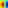
\includegraphics[width=0.25\textwidth]{xsobel.pdf}}
		\subfigure[$G_y$ detektiert horizontale Kanten]{
\includegraphics[width=0.25\textwidth]{ysobel.pdf}}
		\caption{Kantenerkennung durch Sobel-Operatoren}
		\label{fig:sobel}
	\end{figure}
\end{frame}

\begin{frame}
	\frametitle{Kantenerkennung Sobel Filter}
	\begin{figure}
		\centering
		\subfigure{
\includegraphics[width=0.25\textwidth]{wl25.pdf}}
		\subfigure{
\includegraphics[width=0.25\textwidth]{ysobel.pdf}}
		\caption{Ähnlichkeit zu Sobel-Operatoren}
		\label{fig:sobel}
	\end{figure}
	\begin{itemize}
		\item horizontal gespiegelten Sobelfilter $G_y$  
		\item 1. Filter erinnert an Sobelfilter
		\item Faltung mit dem Eingabebild erzeugt ein Gradientenbild
	\end{itemize}
\end{frame}

\begin{frame}
	\frametitle{Ergebnisse normales CNN}
	\begin{figure}
		\subfigure[Genauigkeit]{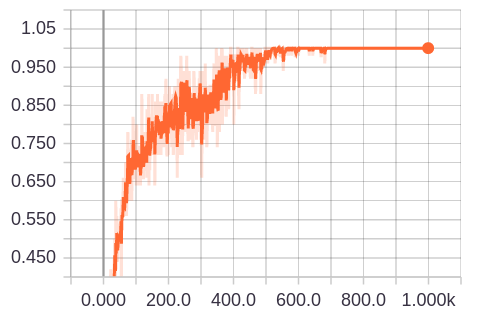
\includegraphics[width=0.4\textwidth]{images/1000_step_accuracy_conv_small.png}}
		\subfigure[Cross Entropy]{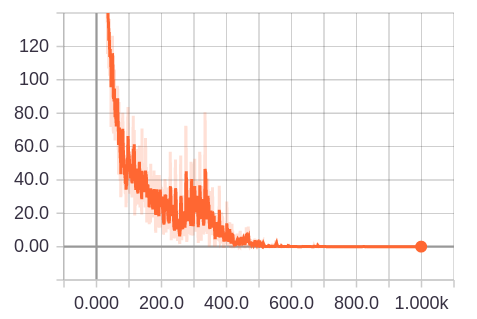
\includegraphics[width=0.4\textwidth]{images/1000_step_cross_entropy_conv_small.png}}
		\label{fig:conv_results}
	\end{figure}
	\begin{itemize}
		\item Trainingsgenauigkeit nach ungefähr 750 Epochen bei 100\%
		\item Testgenauigkeit nach dem Training ungefähr 85\%
		\item Sehr schnelles Training
	\end{itemize}
\end{frame}

\begin{frame}
	\frametitle{Ergebnisse CNN mit Inception Layer}
	\begin{figure}
		\subfigure[Genauigkeit]{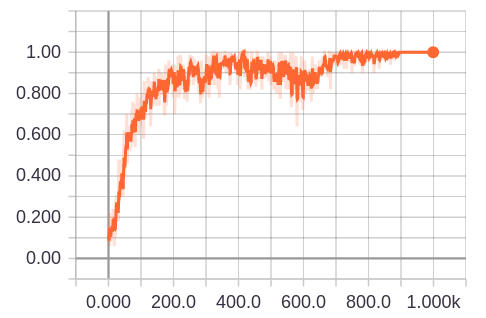
\includegraphics[width=0.4\textwidth]{images/1000_step_accuracy_inception_small.png}}
		\subfigure[Cross Entropy]{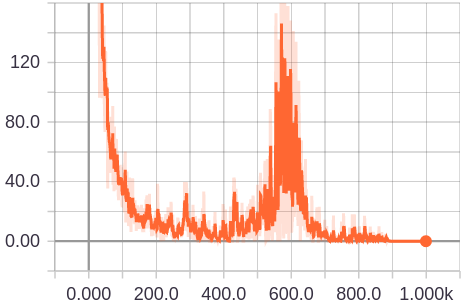
\includegraphics[width=0.4\textwidth]{images/1000_step_cross_entropy_inception_small.png}}
		\label{fig:inception_results}
	\end{figure}
	\begin{itemize}
		\item Trainingsverlauf ähnlich wie bei dem anderen Netz
		\item Gelegentliche Einbrüche der Cross Entropy während Training
		\item Testgenauigkeit auch ungefähr bei 80\%-85\%
		\item Training dauert deutlich länger
	\end{itemize}
\end{frame}

%------------------------------------------------
\section{Diskussion}
%------------------------------------------------

\begin{frame}
	\frametitle{Diskussion}
	\begin{itemize}
		\item Niedrige Genauigkeit im Vergleich zu CNN's mit MNIST Datenset
		\item Grund dafür: Größe des Datensets und fehlerhafte Labels
		\item Hier nur sehr kleine Netze verwendet, Größere Netze sind effektiver für Bildanalyse
		\item Kein Mechanismus um Overfitting zu reduzieren
		\item Netz mit Inception Modul bringt keine besseren Ergebnisse
		\item Vorteil Von Inception: in niedrigen Layern kleine Convolutions, in höheren Layern größere Convolution\\
		$\rightarrow$ In Netz mit nur einem Layer nicht sinnvoll
	\end{itemize}
\end{frame}

%------------------------------------------------
\section{Zusammenfassung und Ausblick}
%------------------------------------------------

\begin{frame}
	\frametitle{Zusammenfassung und Ausblick}
\end{frame}

%------------------------------------------------
%hiernach kommen die besipiele wie man verschiedene sachen in LaTex macht
%------------------------------------------------

\begin{frame}
	\frametitle{Paragraphs of Text}
	Sed iaculis dapibus gravida. Morbi sed tortor erat, nec interdum arcu. Sed id lorem lectus. Quisque viverra augue id sem ornare non aliquam nibh tristique. Aenean in ligula nisl. Nulla sed tellus ipsum. Donec vestibulum ligula non lorem vulputate fermentum accumsan neque mollis.\\~\\
	
	Sed diam enim, sagittis nec condimentum sit amet, ullamcorper sit amet libero. Aliquam vel dui orci, a porta odio. Nullam id suscipit ipsum. Aenean lobortis commodo sem, ut commodo leo gravida vitae. Pellentesque vehicula ante iaculis arcu pretium rutrum eget sit amet purus. Integer ornare nulla quis neque ultrices lobortis. Vestibulum ultrices tincidunt libero, quis commodo erat ullamcorper id.
\end{frame}

\begin{frame}
	\frametitle{Bullet Points}
	\begin{itemize}
		\item Lorem ipsum dolor sit amet, consectetur adipiscing elit
		\item Aliquam blandit faucibus nisi, sit amet dapibus enim tempus eu
		\item Nulla commodo, erat quis gravida posuere, elit lacus lobortis est, quis porttitor odio mauris at libero
		\item Nam cursus est eget velit posuere pellentesque
		\item Vestibulum faucibus velit a augue condimentum quis convallis nulla gravida
	\end{itemize}
\end{frame}

\begin{frame}
	\frametitle{Blocks of Highlighted Text}
	\begin{block}{Block 1}
		Lorem ipsum dolor sit amet, consectetur adipiscing elit. Integer lectus nisl, ultricies in feugiat rutrum, porttitor sit amet augue. Aliquam ut tortor mauris. Sed volutpat ante purus, quis accumsan dolor.
	\end{block}
	
	\begin{block}{Block 2}
		Pellentesque sed tellus purus. Class aptent taciti sociosqu ad litora torquent per conubia nostra, per inceptos himenaeos. Vestibulum quis magna at risus dictum tempor eu vitae velit.
	\end{block}
	
	\begin{block}{Block 3}
		Suspendisse tincidunt sagittis gravida. Curabitur condimentum, enim sed venenatis rutrum, ipsum neque consectetur orci, sed blandit justo nisi ac lacus.
	\end{block}
\end{frame}

\begin{frame}
	\frametitle{Multiple Columns}
	\begin{columns}[c] % The "c" option specifies centered vertical alignment while the "t" option is used for top vertical alignment
		
		\column{.45\textwidth} % Left column and width
		\textbf{Heading}
		\begin{enumerate}
			\item Statement
			\item Explanation
			\item Example
		\end{enumerate}
		
		\column{.5\textwidth} % Right column and width
		Lorem ipsum dolor sit amet, consectetur adipiscing elit. Integer lectus nisl, ultricies in feugiat rutrum, porttitor sit amet augue. Aliquam ut tortor mauris. Sed volutpat ante purus, quis accumsan dolor.
		
	\end{columns}
\end{frame}

\begin{frame}
	\frametitle{Table}
	\begin{table}
		\begin{tabular}{l l l}
			\toprule
			\textbf{Treatments} & \textbf{Response 1} & \textbf{Response 2}\\
			\midrule
			Treatment 1 & 0.0003262 & 0.562 \\
			Treatment 2 & 0.0015681 & 0.910 \\
			Treatment 3 & 0.0009271 & 0.296 \\
			\bottomrule
		\end{tabular}
		\caption{Table caption}
	\end{table}
\end{frame}

\begin{frame}
	\frametitle{Theorem}
	\begin{theorem}[Mass--energy equivalence]
		$E = mc^2$
	\end{theorem}
\end{frame}

\begin{frame}[fragile] % Need to use the fragile option when verbatim is used in the slide
	\frametitle{Verbatim}
	\begin{example}[Theorem Slide Code]
		\begin{verbatim}
		\begin{frame}
		\frametitle{Theorem}
		\begin{theorem}[Mass--energy equivalence]
		$E = mc^2$
		\end{theorem}
		\end{frame}\end{verbatim}
	\end{example}
\end{frame}

\begin{frame}
	\frametitle{Figure}
	Uncomment the code on this slide to include your own image from the same directory as the template .TeX file.
	\begin{figure}
		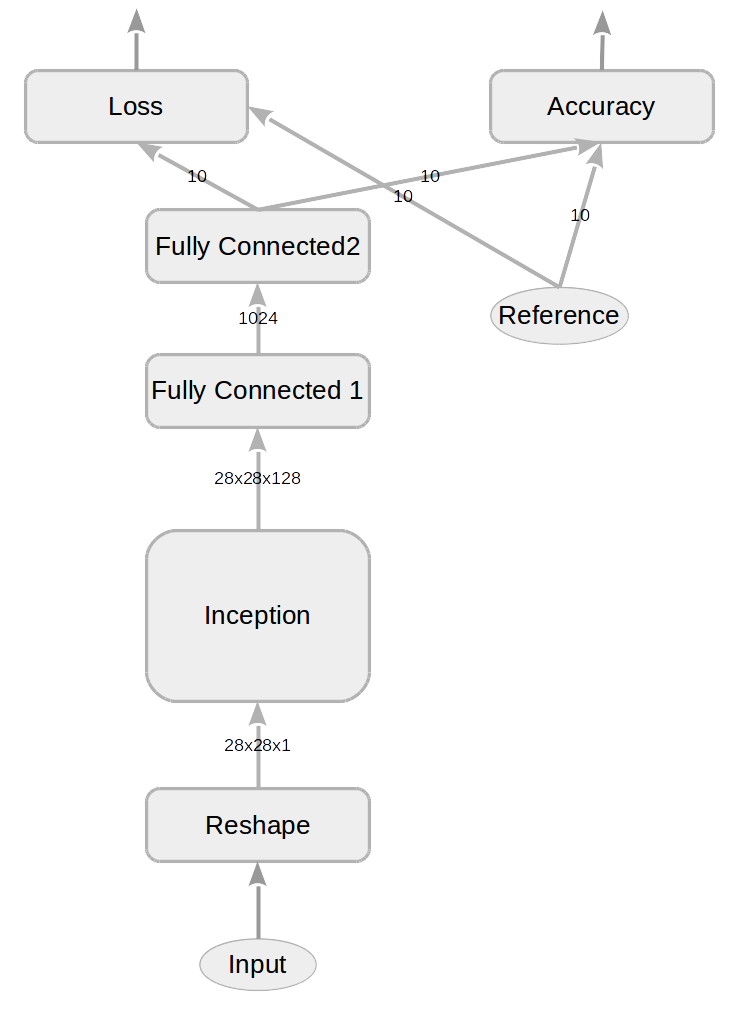
\includegraphics[width=0.4\linewidth]{images/main_graph_inception_reduced.png}
	\end{figure}
\end{frame}

\begin{frame}[fragile] % Need to use the fragile option when verbatim is used in the slide
\frametitle{Citation}
An example of the \verb|\cite| command to cite within the presentation:\\~

This statement requires citation \cite{p1}.
\end{frame}

%------------------------------------------------

\begin{frame}
\frametitle{References}
\footnotesize{
\begin{thebibliography}{99} % Beamer does not support BibTeX so references must be inserted manually as below
\bibitem[Smith, 2012]{p1} John Smith (2012)
\newblock Title of the publication
\newblock \emph{Journal Name} 12(3), 45 -- 678.
\end{thebibliography}
}
\end{frame}

%------------------------------------------------

\begin{frame}
\Huge{\centerline{Vielen Dank für die Aufmerksamkeit}}
\end{frame}

%----------------------------------------------------------------------------------------

\end{document} 